\documentclass[twoside,twocolumn]{article}
\usepackage{amsmath}
\usepackage{blindtext} % Package to generate dummy text throughout this template 
\usepackage{graphicx}
\usepackage{natbib}

\usepackage[sc]{mathpazo} % Use the Palatino font
\usepackage[T1]{fontenc} % Use 8-bit encoding that has 256 glyphs
\linespread{1.05} % Line spacing - Palatino needs more space between lines
\usepackage{microtype} % Slightly tweak font spacing for aesthetics

\usepackage[english]{babel} % Language hyphenation and typographical rules

\usepackage[hmarginratio=1:1,top=32mm,columnsep=20pt]{geometry} % Document margins
\usepackage[hang, small,labelfont=bf,up,textfont=it,up]{caption} % Custom captions under/above floats in tables or figures
\usepackage{booktabs} % Horizontal rules in tables

\usepackage{lettrine} % The lettrine is the first enlarged letter at the beginning of the text

\usepackage{enumitem} % Customized lists
\setlist[itemize]{noitemsep} % Make itemize lists more compact

\usepackage{abstract} % Allows abstract customization
\renewcommand{\abstractnamefont}{\normalfont\bfseries} % Set the "Abstract" text to bold
\renewcommand{\abstracttextfont}{\normalfont\small\itshape} % Set the abstract itself to small italic text

\usepackage{titlesec} % Allows customization of titles
\renewcommand\thesection{\Roman{section}} % Roman numerals for the sections
\renewcommand\thesubsection{\roman{subsection}}
\titleformat{\section}[block]{\large\scshape\centering}{\thesection.}{1em}{} % Change the look of the section titles
\titleformat{\subsection}[block]{\large}{\thesubsection.}{1em}{} % Change the look of the section titles

\usepackage{fancyhdr} % Headers and footers
\pagestyle{fancy} % All pages have headers and footers
\fancyhead{} % Blank out the default header
\fancyfoot{} % Blank out the default footer
\fancyhead[C]{FYS4150 $\bullet$ Project 2 $\bullet$ Oktober 2016} % Custom header text
\fancyfoot[RO,LE]{\thepage} % Custom footer text

\usepackage{titling} % Customizing the title section

\usepackage{hyperref} % For hyperlinks in the PDF

%----------------------------------------------------------
%  COMMANDS
%---------------------------------------------------------

\newcommand{\nl}{
	
	\medskip
	\noindent
}
%--------------------------------------------



%----------------------------------------------------------------------------------------
%	TITLE SECTION
%----------------------------------------------------------------------------------------

\setlength{\droptitle}{-4\baselineskip} % Move the title up

\pretitle{\begin{center}\Huge\bfseries} % Article title formatting
	\posttitle{\end{center}} % Article title closing formatting
\title{FYS4150 - Project 1} % Article title
\author{%
	\textsc{Vegard R�nning \& Heine H. Ness \& Sindre R. Bilden} \\[1ex] % Your name
	\normalsize University of Oslo \\ % Your institution
	\normalsize \href{mailto:vegarduio@gmail.com}{vegarduio@gmail.com}\ ; \href{mailto:h.h.ness@fys.uio.no}{h.h.ness@fys.uio.no}\ ; \href{mailto:s.r.bilden@fys.uio.no}{s.r.bilden@fys.uio.no}\\% Your email address
	\footnotesize \href{https://github.com/sindrerb/FYS4150-Collaboration/tree/master/Doc/Project2}{github.com/sindrerb/FYS4150-Collaboration/tree/master/Doc/Project2}
	%\and % Uncomment if 2 authors are required, duplicate these 4 lines if more
	%\textsc{Jane Smith}\thanks{Corresponding author} \\[1ex] % Second author's name
	%\normalsize University of Utah \\ % Second author's institution
	%\normalsize \href{mailto:jane@smith.com}{jane@smith.com} % Second author's email address
}
%----------------------------------------------------------------------------
\date{\today} % Leave empty to omit a date
\renewcommand{\maketitlehookd}{%
	\begin{abstract}
		
		
		
	\end{abstract}
}

%----------------------------------------------------------------------------

\begin{document}
	
	% Print the title
	\maketitle
	
	%----------------------------------------------------------------------------
	%	ARTICLE CONTENTS
	%----------------------------------------------------------------------------
	
	\section{Introduction}
	\lettrine[nindent=0em,lines=2]{Q}uantum mechanical systems with one particle, like a quantum dot, is often possible to approximate to simple systems and solve analytically. Systems containing two or more paricles complicates the problem drastically and is often not possible to solve in the same way as for a single paricle system. By numerical methods, a close approximation may be achieved, and may be used to confirm experimental results or used as an experiment by itself. This project consists of two main parts where the first is solving the Shroedinger equation (SE) numerically for one particle in a three dimensional harmonic oscillator(HO) potential. The second part is to introduce a second particle and solve the system with and without Coulomb interactions. The schrodinger equation is solved by Jacobi's method as an eigenvalue equation rewriting it in a discretized form.
	
	%----------------------------------------------------------------------------
\section{Methods}
	
\subsection{Jacobi's method}
The Jacobi's method uses Jacobi's rotation matrix $\hat{S}$ a number of times to turn all vectors in a symmetric or hermittian matrix $\hat{A}$ so that it become a diagonal matrix $\hat{D}$.
	
\begin{equation*}
\hat{S}^T_n\hat{S}^T_{n-1}\cdots\hat{S}^T_1\hat{A}\hat{S}_1\cdots\hat{S}_{n-1}\hat{S}_n = \hat{D}
\end{equation*}
	
\noindent
The rotation matrix $\hat{S}_i$ has the form of an identity matrix with $c = \cos(\theta)$ and $s = \sin(\theta)$ in a symmetric fashion inside depending on which two elements in $\hat{A}$ is to be rotated. $n$ depends on the number of rotations needed to transform $\hat{A}$ to $\hat{D}$.
	
	\begin{equation*}
	\hat{S} = \begin{bmatrix}
	1 & 0 & & \cdots & & & 0 \\
	0 & \ddots &  &  & & & \\
	&  & c & \cdots & s & &\\
	\vdots & & \vdots & \ddots & \vdots & &\vdots\\
	& & -s & \cdots & c & &\\
	& & & & &\ddots & 0\\
	0 & & & \cdots & & 0 & 1
	\end{bmatrix}
	\end{equation*}
	
	If $\hat{A}$ is composed of elements $a_{ij}$ and matrix $\hat{B}$ of elements $b_{ij}$. 
	One rotation $\hat{S}^T\hat{A}\hat{S} = \hat{B}$ can be done with an algorithm. 
	\nl
	First the largest element$a_{kl}$ has to be located, then the new element will be set to zero $b_{kl} = (a_{kk}-a_{ll})cs + a_{kl}(c^2-s^2) = 0$. For $b_{kl} = 0$ the equation $(a_{kk}-a_{ll})cs + a_{kl}(c^2-s^2) = 0$ is solved using $\Gamma = \frac{a_{ll} - a_{kk}}{2a_{kl}}$ by the second order polynomial $t^2 + 2\Gamma t-1 = 0$. Here $t = \tan(\theta) = \frac{s}{c}$. This gives solutions for the trigonometrical expessions $t = -\Gamma\pm \sqrt{1+\Gamma^2}$ , $s = tc$ and $c = \frac{1}{\sqrt{1 + \Gamma^2}}$. To avoid problems where $\Gamma$ gets large and possible loss of numerical presission we rewrite $t = \frac{1}{\Gamma + \sqrt{1+\Gamma^2}}$.
	\nl
	Rotation algorithm is solved with the prevusly given solutions for $t$,$c$ and $s$. Here $i$ is the iteration variable and $k$ and $l$ are parameter belonging to the element in rtotation:
	\begin{align*}
	&b_{ii} = a_{ii} &|i\neq k,l\\
	&b_{ik} = a_{ik}c - a_{il}s &|i\neq k,l\\
	&b_{il} = a_{il}c + a_{ik}s &|i\neq k,l\\
	&b_{kk} = a_{kk}c^2 - 2a_{kl}cs + a_{ll}s^2&\\
	&b_{ll} = a_{ll}c^2 + 2a_{kl}cs + a_{kl}s^2&\\
	&b_{kl} = b_{lk} = 0&
	\end{align*}
	
\subsection{Unit tests}
A unit test is a small piece of code that tests parts of a program for calculation errors. This to ensure that the program runs as expected and delivers correct results throughout the program. The unit tests we have used in this assignment are as follows.
	
\subsubsection{Orthogonality test}
	
The Jacobi method preforms orthogonal or unitary transformations to the matrix it operates on. That means the orthogonality of each column in a matrix $\hat{A}$ is conserved.\nl

If $\hat{A}$ is a orthogonal matrix with orthogonal column vectors $\hat{A} = [\vec{a_1} \vec{a_2} \cdots \vec{a_n}  ]$ the dot product of any column vector can be described by a Kronecker delta $\delta_{ij}$.
	
	\begin{align*}
	\vec{a_i}^T \vec{a_j} = \delta_{ij} =
	\begin{cases}
	1|i=j\\
	0|i\neq j
	\end{cases}
	\end{align*}
	
	For a transformation done by a matrix $\hat{S}$ to be unitary any column all vectors $\vec{w_i}$ produced by the transformation $\hat{S}\vec{v_i} = \vec{w_i}$ must also be orthogonal.
	
	\begin{align*}
	&\vec{w_i^T}\vec{w_j} = (\hat{S}\vec{v_i})^T\hat{S}\vec{v_j} = \hat{S}^T\vec{v_i}^T\hat{S}\vec{v_j} = \\ &\vec{v_i}^T\hat{S}^T\hat{S}\vec{v_j} = \vec{v_i}\vec{v_j} = \delta_{ij}
	\end{align*}
	
\subsubsection{Normality test}	
Since the Jacobi method preforms unitary transformations to the matrix it operates on, the normality is conserved if the columns of $\hat{A}$ is normalized.\nl
This project is using Jacobi rotation on the identity matrix wich is normalized by definition. Introducing the criteria $$col_i(\hat{A})^T\cdot col_i(\hat{A})=1$$ gives a brief indication of the conservation of normality.
	%----------------------------------------------------------------------------
\section{Implementation}
A quantum dot may be approximated to a three dimentional HO-potential. By assuming shperical symmetry the radial part the SL may be rewritten to
\begin{align*}
		&-\dfrac{\hbar^2}{2 m} \left ( \dfrac{1}{r^2} \dfrac{d}{dr} r^2 \frac{d}{dr} - \dfrac{l (l + 1)}{r^2} \right )R(r) + V(r) R(r)\\ 
		&= E R(r).
		\end{align*}
Where the potential $V(r)$ is known by the HO-potential $\frac{1}{2}kr^2$, with $k=m\omega^2$ and the quantum number $l$ describe the orbital momentum of the electron.
The energies and oscillator frequency is given by
\begin{align*}
E_{nl} = \hbar\omega\left(2n+l+ \dfrac{3}{2} \right)
		\end{align*}
		where $n\in \mathbb N$, $l\in \mathbb N$ and $r \in [0,\infty)$. By rewriting $R(r)$ as $rR(r) = u(r)$ we get
		\begin{align*}
		-\dfrac{\hbar^2}{2 m} \frac{d^2}{dr^2} u(r) + \left ( V(r) + \dfrac{l (l + 1)}{r^2}\dfrac{\hbar^2}{2 m} \right ) u(r)  = E u(r)
		\end{align*}
		The expression can be further simplified by introducing the dimensionless variable $\rho = \frac{1}{\alpha}r$, setting $V(\rho) = \frac{1}{2}k\alpha^2\rho^2$, multiply with $\frac{2m\alpha^2}{\hbar^2}$ and set $l=0$ so that
		\begin{align*}
		-\frac{d^2}{d\rho^2} u(\rho) +\underbrace{ \frac{mk}{\hbar^2} \alpha^4}_{I}\rho^2u(\rho)  = \underbrace{\frac{2m\alpha^2}{\hbar^2}E}_{II}u(\rho)
		\end{align*}
		and finally setting I $=1$ and defining II $=\lambda$ the final form of the SL for one electron in a HO-potential can be written as
		\begin{align}
		-\frac{d^2}{d\rho^2} u(\rho) + \rho^2u(\rho)  = \lambda u(\rho)\label{eq:dimless}
\end{align}
Equation \ref{eq:dimless} may be discretized and solved nummerically as a matrix eigenvalue problem.
\begin{equation}
-\frac{u_{i+1}-2u_i+u_{i-1}}{h^2}+V_iu_i = \lambda u_i
\end{equation}
Were $V_i=\rho_i^2$. The problem may be rewritten to $\hat{H}\hat{u}=\lambda\hat{u}$ were $\hat{H}$ is a tridiagonal matrix with center diagonal $d_{ii}=\frac{2}{h^2}+V_i$ and the upper diagonal equal to the lower diagonal equal to $e_{ij}=\frac{-1}{h^2}$. This matrix eigenvalue problem may be solved by Jacobi's method.\nl

By introducing another electron to the system, the system includes two particles in the potential and the interactions between them.
This may be solved by splitting the problem into relative cooridnates $r=r_1-r_2$ and $R=r_1+r_2$.\\

!SKRIV MER HER!\\

Tests of conserved orthogonality and normality was done in forehand to ensure that the algorithm was correct. Later a convergence test of the number of iterations was done to weight the accuaracy and computational time. The algortihm was set to solve the schr\o edinger equation with $\omega_r$ equal to $0.01,0.5,1$ and $5$. Both with and without columb interactions.
\section{Results and discussion}
The jacobian method requires many iterations in order to reach a satisfying accuaracy of the energies. Table \ref{tbl:convergence} from the convergence test of meshpoints indicates that $N=500$ is a minimum requirement for a four digit accuaracy but results also in a high computational time. Figure \ref{fig:iterations} shows the number of iterations for a given set of meshpoints, assumed to be proportional to computation time.
A number of meshpoints $N=400$ results in a high enough accuaracy for the purpose of this experiment and reducing the computational time drastically.\vfill

\begin{table}[p]
\centering
\begin{tabular}{|l|l|l|l|}\hline
$N$ & $\lambda_0$ & $\lambda_1$ & $\lambda_2$\\ \hline
10 & 2.68672 & 6.11302 & 11.0574\\
50 & 2.98745 & 6.93692 & 10.8453\\
100& 2.99687 & 6.98432 & 10.9617\\
200& 2.99916 & 6.99610 & 10.9904\\
300& 2.99961 & 6.99828 & 10.9958\\
400& 2.99986 & 6.99903 & 10.9976\\
500& 2.99993 & 6.99937 & 10.9986\\\hline
\end{tabular}
\caption{Table showing the three lowest computed eigenvalues $\lambda$ with $N$ meshpoints, in comparment to the exact $\lambda_0=3$,$\lambda_1=7$ and $\lambda_2=11$.}\label{tbl:convergence}
\end{table}
\begin{figure}[p]
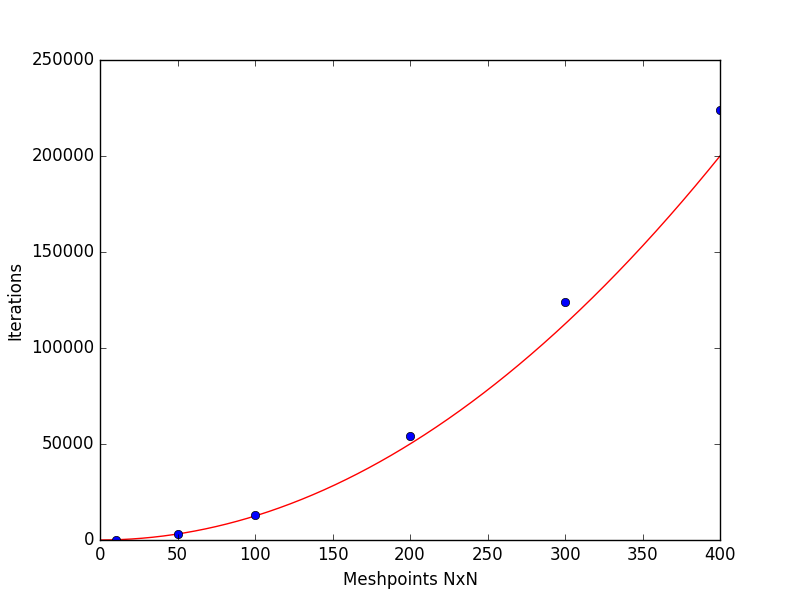
\includegraphics[width=0.5\textwidth]{figures/iterations.png} 
\caption{Graph over the number of iterations for a given set of meshpoints $N$. The red line is proportional to $N^2$ as comparement.}\label{fig:iterations}
\end{figure}
\begin{figure}[p]
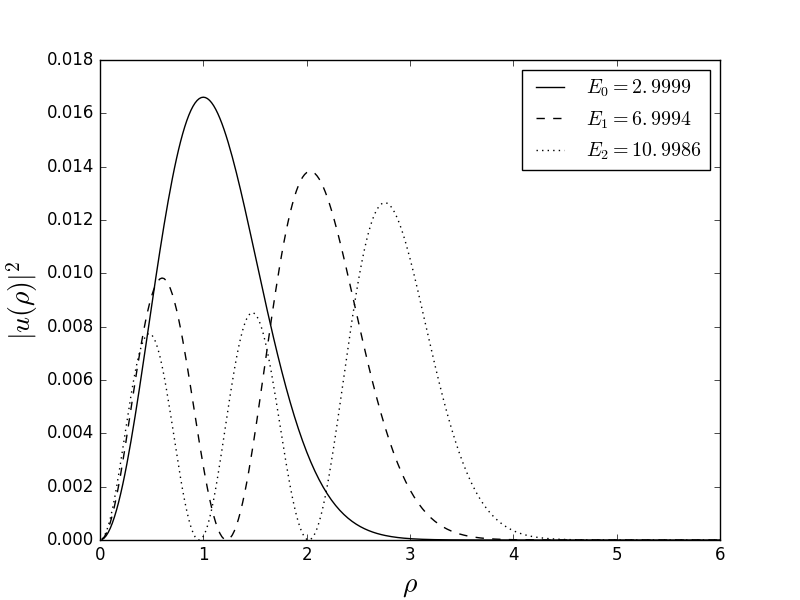
\includegraphics[width=0.5\textwidth]{../report/figures/eigenvecs123.png} 
\caption{The first three eigenstates with their respective eigenstates in a harmonic oscillator with one particle, computed with $N=500$ meshpoints.}\label{fig:eigenstates}
\end{figure}

Results from the computation of the two particle systems is given in Figure \ref{fig:fq001} $-$ \ref{fig:fq500}, where it is a clear correspondance between the $\omega_r$ and the columb interactions. A high $\omega_f$ results in a narrow potential and a confinement of the electrons, in this narrow potential the columb interactions was thought to give a great impact on the wavefunction but Figure \ref{fig:fq500} contradicts this hypothesis. Figure \ref{fig:fq001} does also show sn unexpected behaviour where the columb interaction has a greater impact in the electrons than expected. The behaviour may be explained by the fact that $V_{Columb}=\frac{\beta}{r}$ diverge while $r$ goes to zero. In a narrow potential, the columb interactions is large but does not  overpower the confinement of the potential. While widening the potential, the confinement decreases more rapidly than the columb interactions.

\begin{figure}[p]
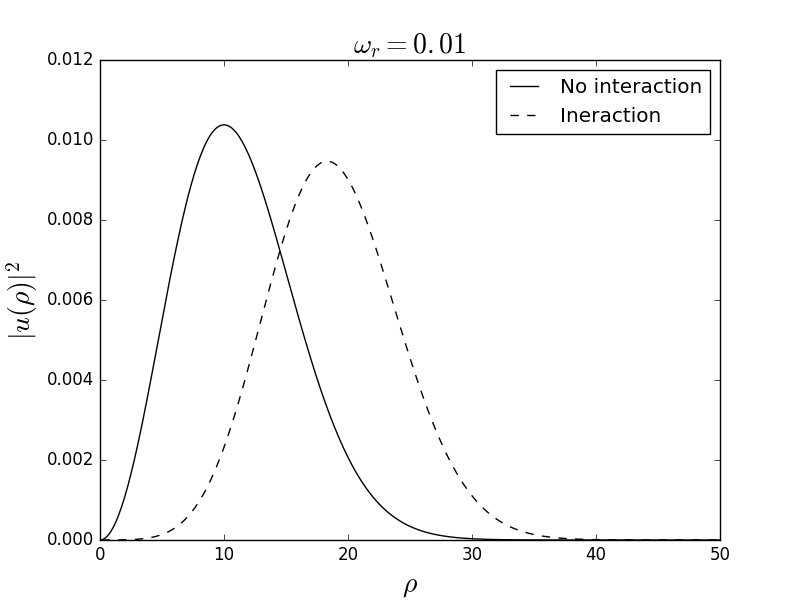
\includegraphics[width=0.45\textwidth]{../report/figures/freq001.png} 
\caption{Comparison of the wavefunction with and without columb interactions in a HO-potential where $\omega_r=0.01$}\label{fig:fq001}
\end{figure}
\begin{figure}[p]
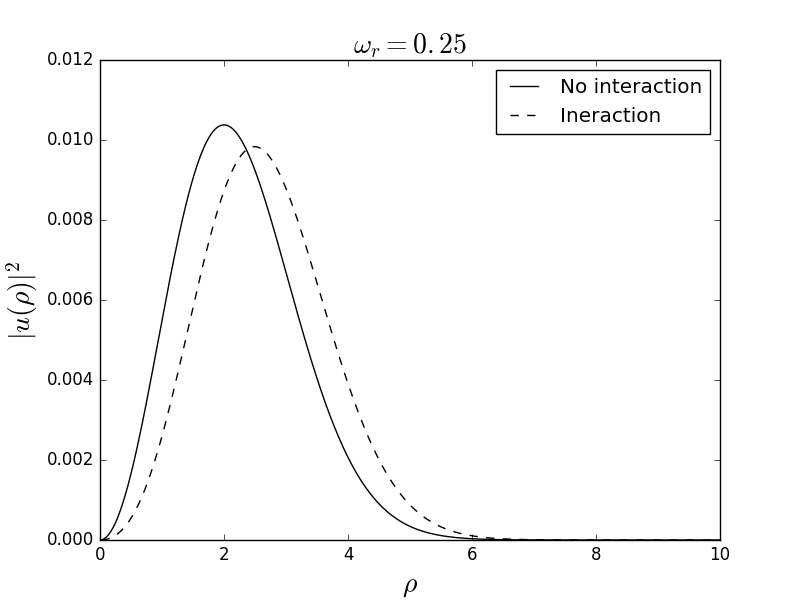
\includegraphics[width=0.45\textwidth]{../report/figures/freq025.png} 
\caption{Comparison of the wavefunction with and without columb interactions in a HO-potential where $\omega_r=0.25$}\label{fig:fq025}
\end{figure}
\begin{figure}[p]
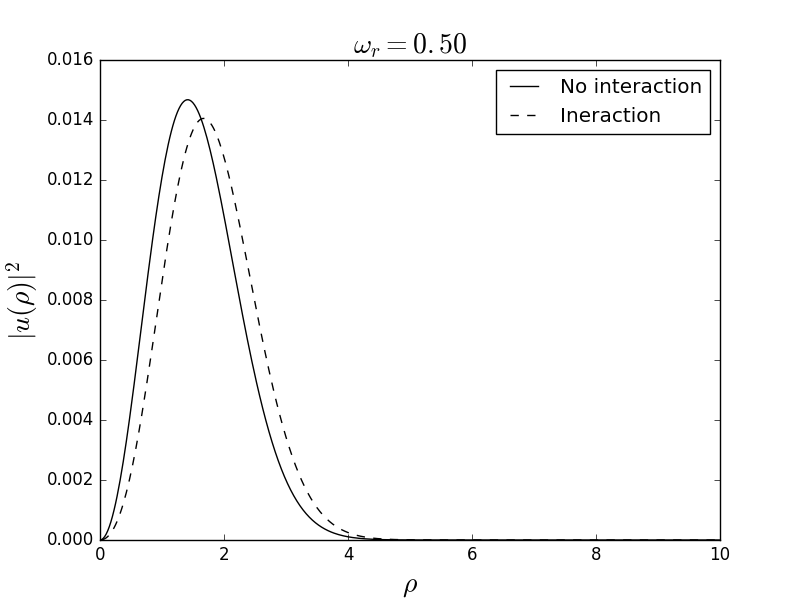
\includegraphics[width=0.45\textwidth]{../report/figures/freq050.png} 
\caption{Comparison of the wavefunction with and without columb interactions in a HO-potential where $\omega_r=0.5$}\label{fig:fq050}
\end{figure}
\begin{figure}[p]
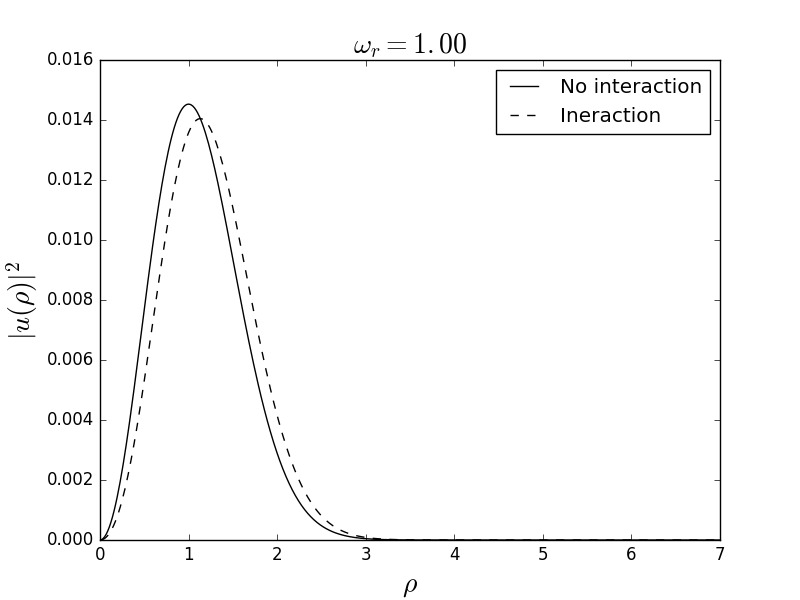
\includegraphics[width=0.45\textwidth]{../report/figures/freq100.png} 
\caption{Comparison of the wavefunction with and without columb interactions in a HO-potential where $\omega_r=1.00$}\label{fig:fq100}
\end{figure}
\begin{figure}[p]
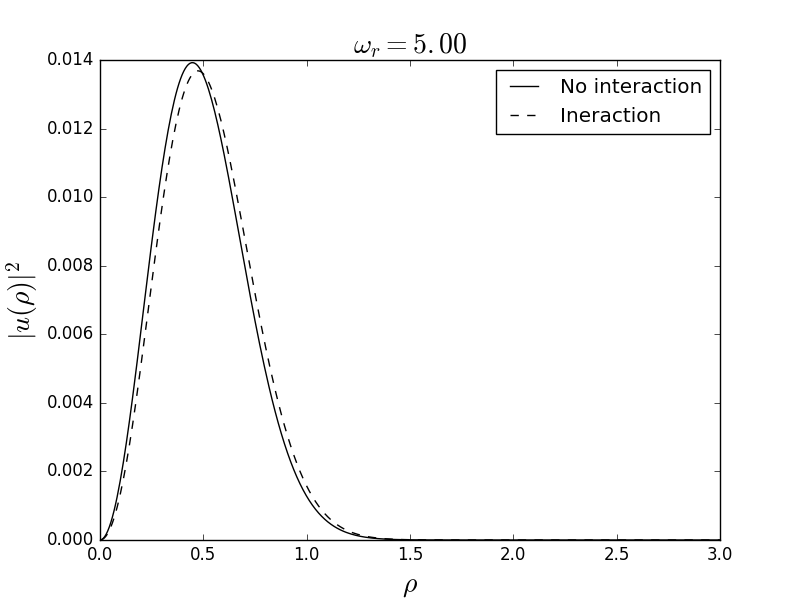
\includegraphics[width=0.45\textwidth]{../report/figures/freq500.png} 
\caption{Comparison of the wavefunction with and without columb interactions in a HO-potential where $\omega_r=5.00$}\label{fig:fq500}
\end{figure}	%----------------------------------------------------------------------------
\section{Summary and Conclusion}

	%----------------------------------------------------------------------------
	%\twocolumn[{%
	%	\bibliography{ref.bib}{}
	%	\bibliographystyle{plain}
	%}]
\end{document}